\documentclass[12pt, a4paper,fleqn]{article}
\usepackage[utf8]{inputenc} %indicates the encoding of the document
\usepackage{multicol}
\usepackage{multirow}
\usepackage{graphicx}
\usepackage{amsmath}
\usepackage{amsfonts} 
% or 
\usepackage{amssymb}
\usepackage{authblk}
\usepackage[document]{ragged2e}
\usepackage{geometry}

\title{CSE 300: Online Assignment}
\author{Md Shamsuzzoha Bayzid, Mahjabin Nahar, Md Shariful Islam Bhuyan and Md Saidur Rahman}
\date{June 2021}
\begin{document}
\maketitle

\section{Introduction}
This assignment has been designed to assess the preparation of the students in writing scientific articles using \LaTeX. This assignment covers a variety of components that are commonly used in scientific manuscripts.
    \subsection{Equations}
    Let $a_0$ $a_n$ and $b_n$ are the terms of a series. Therir definitions are given in Eqn. \ref{eq:1}.
    \begin{equation}\label{eq:1}
        \begin{aligned}[b]
            a_0 &= \frac{1}{\pi} \int^{-\pi}_{\pi} f(x) dx \\
            a_n &= \frac{1}{\pi} \int^{-\pi}_{\pi} \cos nx \,dx = \frac{1}{\pi} \int^{-\pi}_{\pi} x^2 \cos nx \,dx \\
            b_n &= \frac{1}{\pi} \int^{-\pi}_{\pi} \sin nx \,dx = \frac{1}{\pi} \int^{-\pi}_{\pi} x^2 \sin nx \,dx \\
        \end{aligned}
    \end{equation}
    \subsection{Tables}
    We wish to place the Table at the bottom of the page.
    \subsection{Figures}
    We intend to put Figure \ref{fig:1} at the top of a page.\pagebreak
    \begin{figure}[t!]
        \centering
        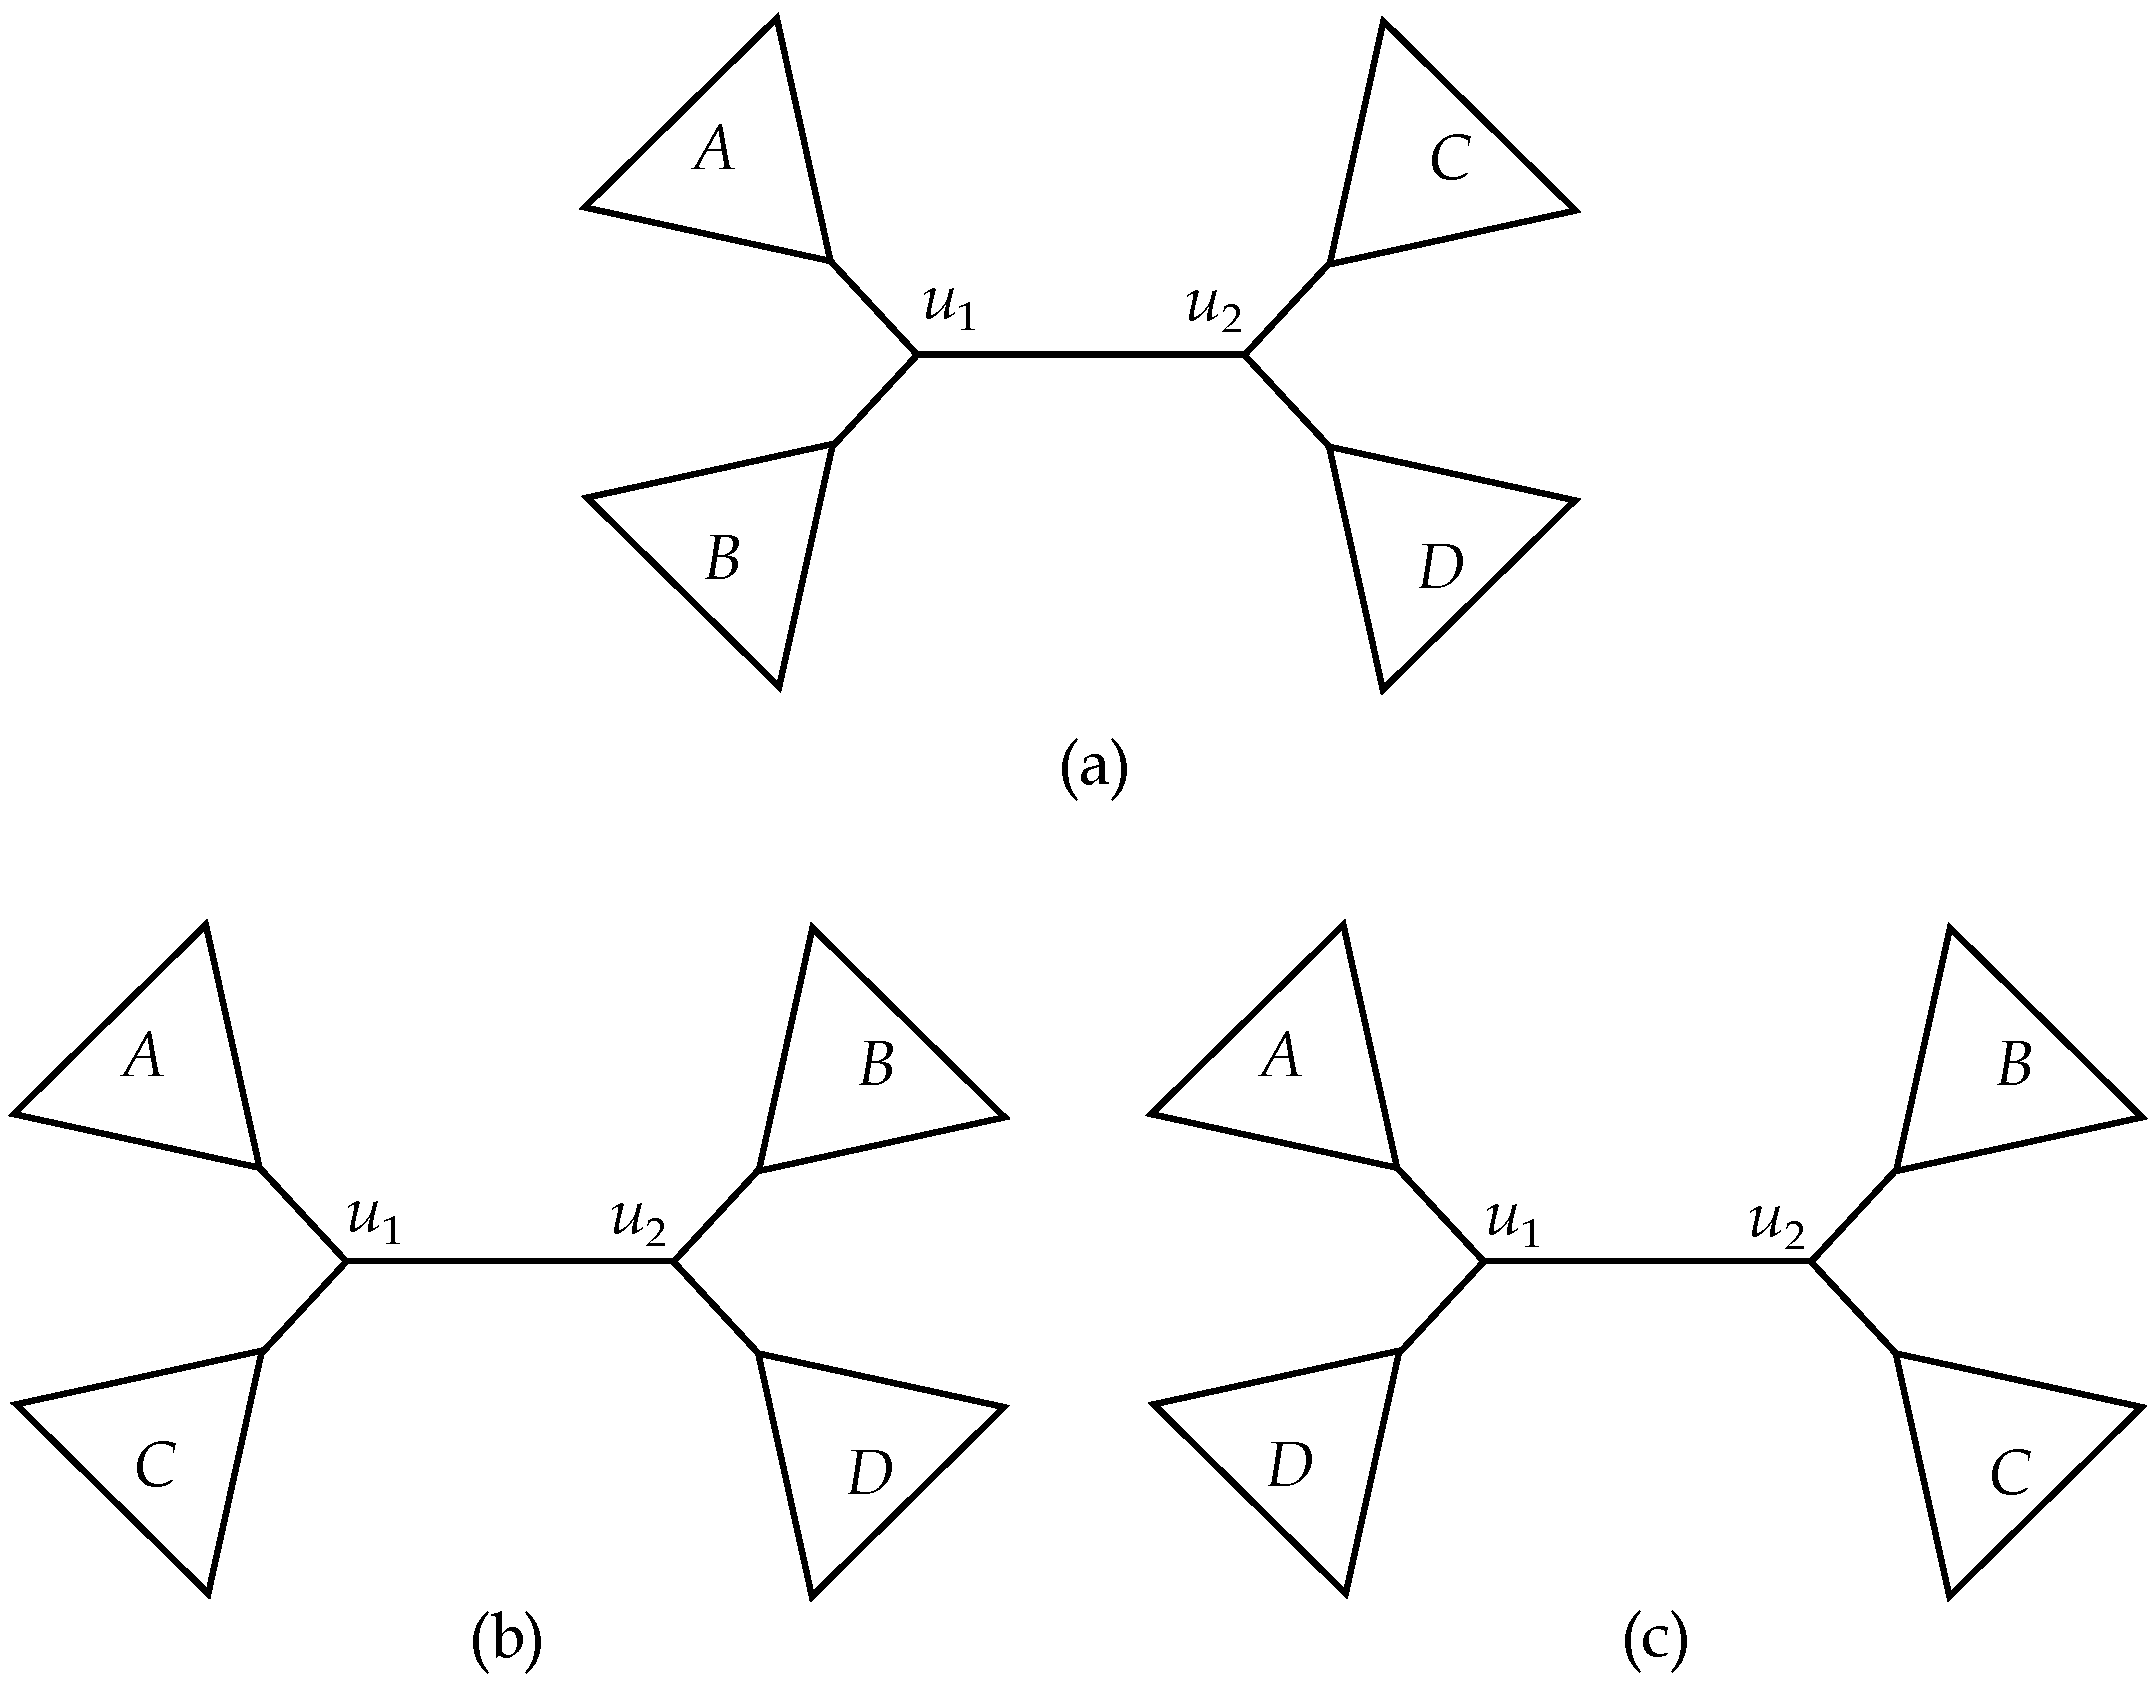
\includegraphics[width=0.60\linewidth]{Figure3.pdf}
        \caption{\label{fig:1}\textbf{Side by side same figure}}
    \end{figure}
\section{Conclusions}
The major objectives of this assignment are listed below (please do not ignore the font sizes)
    \begin{itemize}
     \item {\huge{To assess the ability of the students in preparing manuscripts in \LaTeX}}
     \item {\large{To see if the students have adequately practiced different aspects of writing in \LaTeX}}
\begin{table}[h]
\centering
\begin{tabular}{|l||l|l|l|}
\hline
\multicolumn{4}{|c|}{Item List} \\ \hline
Item \hspace{3mm} Name \hspace{3mm} or & \multirow{2}{*}{ALPHA 2 Code\hspace{4mm}} & \multicolumn{1}{l|}{\multirow{2}{*}{ALPHA 3 Code\hspace{4mm}}} & \multirow{2}{*}{Numerical Code} \\
Product Name &  & \multicolumn{1}{l|}{} &  \\ \hline
Item001 & AF & AFG &  \begin{tabular}{|c|}\hline 004 \\ \hline \end{tabular} \\
Item002 & AX & ALA &  \begin{tabular}{|c|}\hline 008 \\ \hline \end{tabular} \\
Item003 & AL & ALB &  \begin{tabular}{|c|}\hline 009 \\ \hline \end{tabular} \\
Item004 & DZ & DZA &  \begin{tabular}{|c|c|c|} \cline{1-3} 012 & 013 & 024 \\ \end{tabular} \\
\hline \hline
Item005 & AS & ASM &  \begin{tabular}{|c|} \hline 016 \\ \hline \end{tabular} \\
Item006 & AD & AND &  \begin{tabular}{|c|c|}\cline{1-2} 010 & 020 \\ \hline \end{tabular} \\
Item007 & AO & AGO &  \begin{tabular}{|c|c|} \cline{1-2} 024 & 025 \\ \hline \end{tabular} \\
\hline\hline \hline
\end{tabular}
\end{table}
\pagebreak
    \item{To see if the students can add various basic components (e.g., tables, figures, equations) to a \LaTeX manuscript.
}
    \item{\small{To see if the students can leverage the available materials (both offline and online) to do something which has not explicitly been taught in the class.}}
    \end{itemize}
\end{document}
